\documentclass[a4paper,10pt]{article}

\usepackage[a4paper,margin=1in]{geometry}
\usepackage{multicol}       % For multiple columns
\usepackage{graphicx}       % For including images if needed
\usepackage{parskip}        % No paragraph indent, adds space between
\usepackage{titlesec}       % For section title formatting
\usepackage{mathptmx}
\usepackage{amsmath}
\usepackage{subcaption}
\usepackage{float}  % for [H] placement
\usepackage{amsmath,amssymb}
\usepackage[authoryear]{natbib}
\usepackage[colorlinks=true, citecolor=blue, linkcolor=black, urlcolor=blue]{hyperref}


% Optional: Customize section formatting
\titleformat{\section}{\large\bfseries}{\thesection}{1em}{}
\titleformat{\subsection}{\normalsize\bfseries}{\thesubsection}{1em}{}

\begin{document}

\begin{center}
    {\Large \textsc{Disentangling the Components of the Milky Way}}\\[0.2cm]
    {\textsc{Inferring the Structure of the Milky Way in Phase-Space Using Gaussian Mixture Modelling with Extreme Deconvolution}}\\[0.2cm]
    Raunaq Singh Rai \quad | \quad MPhil Data Intensive Science \quad | \quad University of Cambridge
\end{center}

\begin{multicols}{2}
% Start of two-column content

\subsection*{Motivation and Scientific Justification}

A central question in Galactic Archaeology is \emph{when} the Milky Way’s disc first settled.  
Standard models place disc formation after the interstellar medium had already been enriched, implying few (if any) stars on disc-like orbits below $[\mathrm{Fe/H}] \simeq -1.5$.  
Finding even a small, coherent very-metal-poor (VMP) disc would therefore overturn the “late–disc’’ paradigm and force a rethink of in-situ versus accreted growth.

Zhang et al.\ (2024) \cite{zhang2024existencemetalpoordiscmilky} tackled this problem with Extreme-Deconvolution Gaussian Mixture Modelling (XD-GMM) of Gaia DR3 red giants and reported \textit{no} cold VMP disc.  
Their analysis, however, did not separate stars by $\alpha$-abundance, a key tracer of formation timescale.

We reproduce their metallicity-binned XD-GMM on the same bright-RGB catalogue and extend it by splitting the sample into high- and low-$\alpha$ sequences (Viswanathan et al.\ 2024 \cite{Vis2024}).  
For each chemical branch we fit XD-GMMs in successive metallicity bins, letting the Bayesian Information Criterion choose the minimum number of Gaussian components.  
Comparing the weights and kinematics of these components lets us decide whether any disc-like signal at low metallicity is genuine or an artefact of noise, misclassification, or accreted debris.

By tightening the chemical and kinematic tests in this way, we provide a more robust verdict on early disc formation and thereby refine constraints on the Milky Way’s assembly history.

\subsection*{Methodology}

We use a cleaned sample of red giant branch (RGB) stars from Gaia DR3, with metallicities and $\alpha$-abundances from Andrae et 
al. Catalogue~\cite{Andrae2023} and the Li et al. Catalogue~\cite{Li2024}, and distances from the Bailer-Jones et al. 
Catalogue~\cite{BailerJones2021}. As analysis largely depends on the accuracies of metallicities regions of high extinction, 
where XP spectra is known to be bias, are excluded with the sacrifice of losing a large proportion of RGB stars from subsequent anaysis..

The velocity distribution $(v_R, v_\phi, v_z)$ is modelled using Extreme-Deconvolution Gaussian Mixture Modelling (XD-GMM) \cite{Bovy2011}\cite{pygmmis}, 
which accounts for observational uncertainties. We bin stars by metallicity and use the Bayesian Information Criterion (BIC) to determine the 
number of Gaussian components per bin. This allows us to identify structure without over fitting and introducing too many gaussians.


We extend the original method by splitting the sample into high- and low-$\alpha$ sequences \citep{Vis2024}, fitting separate 
XD-GMMs to each. By inspecting the component weights and kinematic properties, we quantify the emergence of rotational support 
and assess the presence of disc-like populations across both chemical tracks.

\subsection*{Key Findings}

\begin{figure}[H]
  \centering
  \begin{subfigure}[t]{0.24\linewidth}
    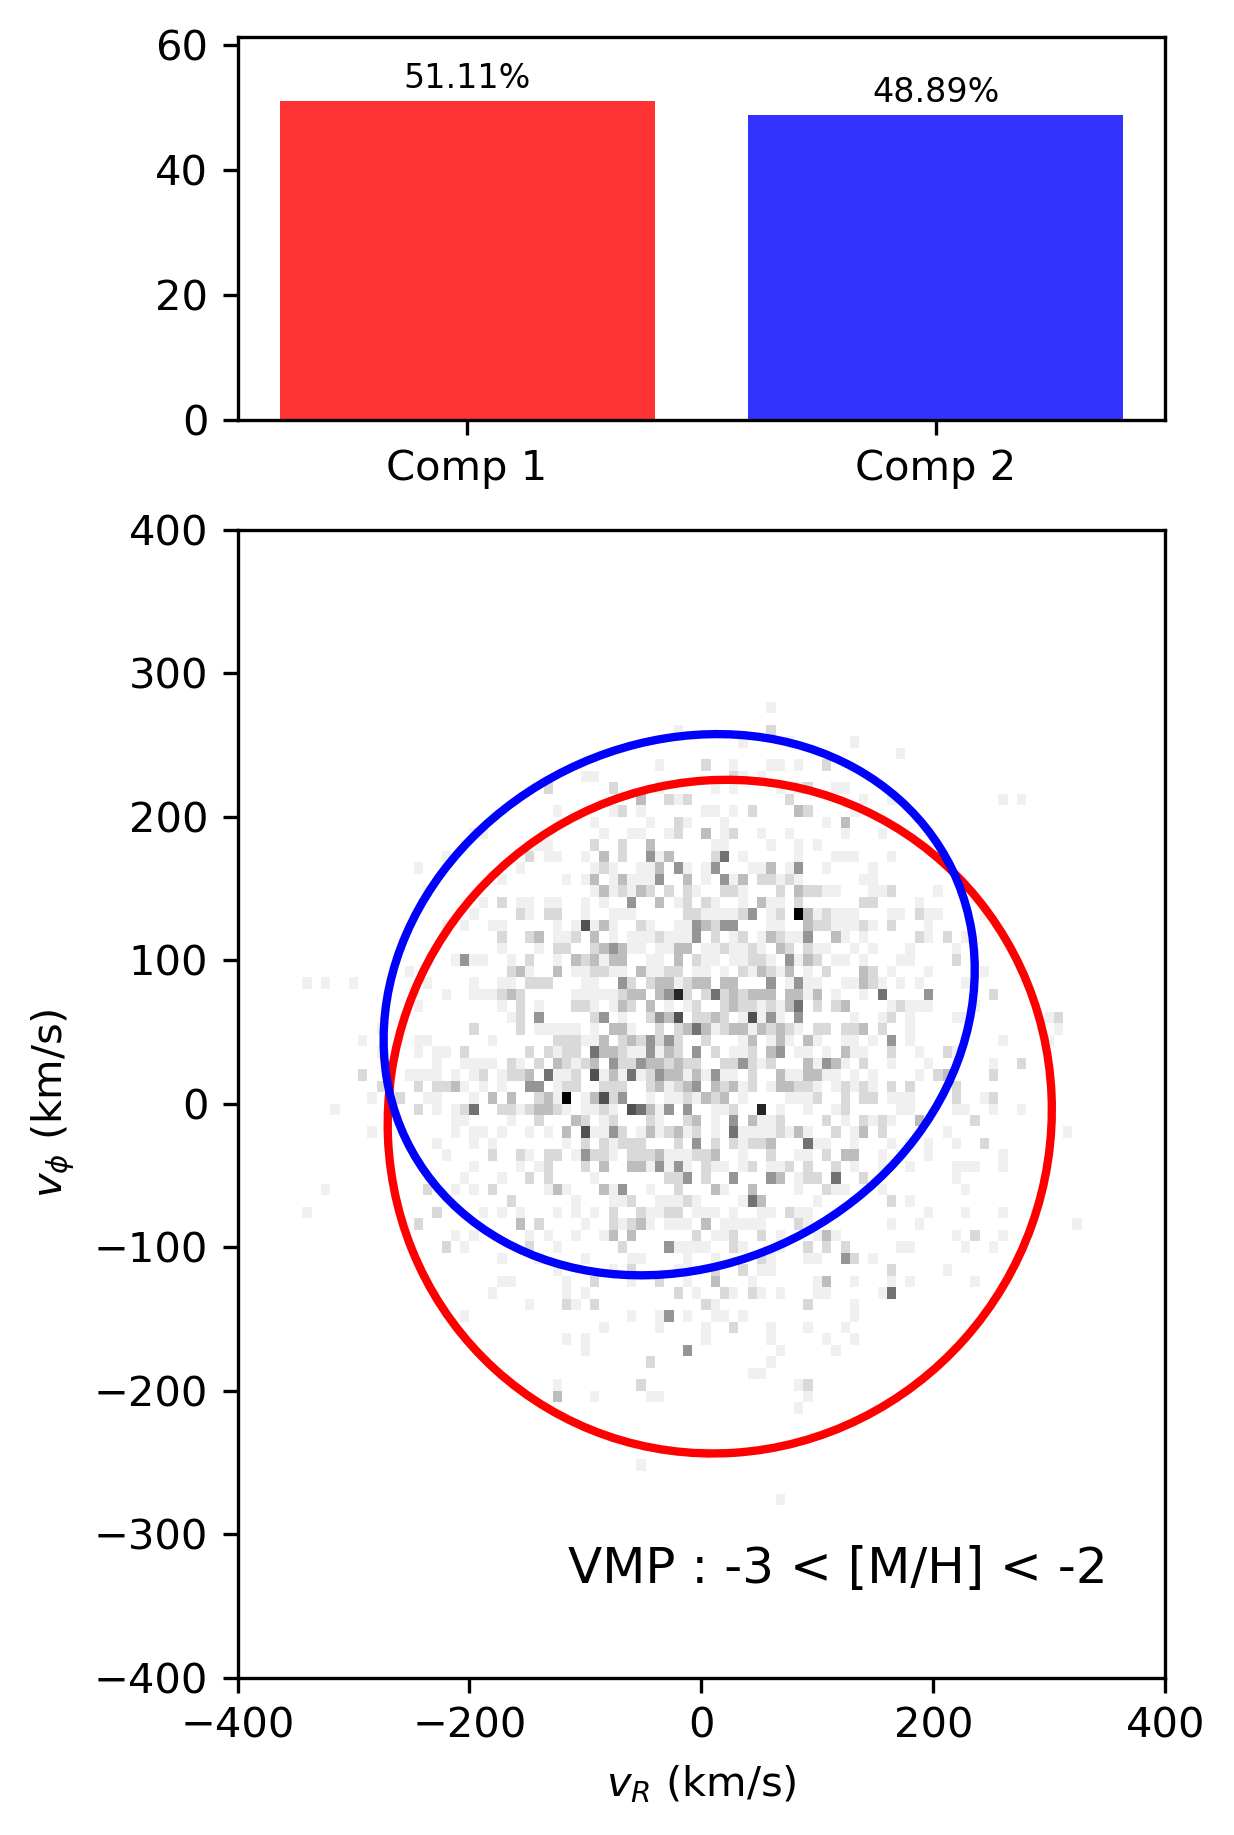
\includegraphics[width=\linewidth]{../figures/gmm_VMP.png}
    \caption{VMP}
    \label{fig:gmm_vmp}
  \end{subfigure}
  \hfill
  \begin{subfigure}[t]{0.24\linewidth}
    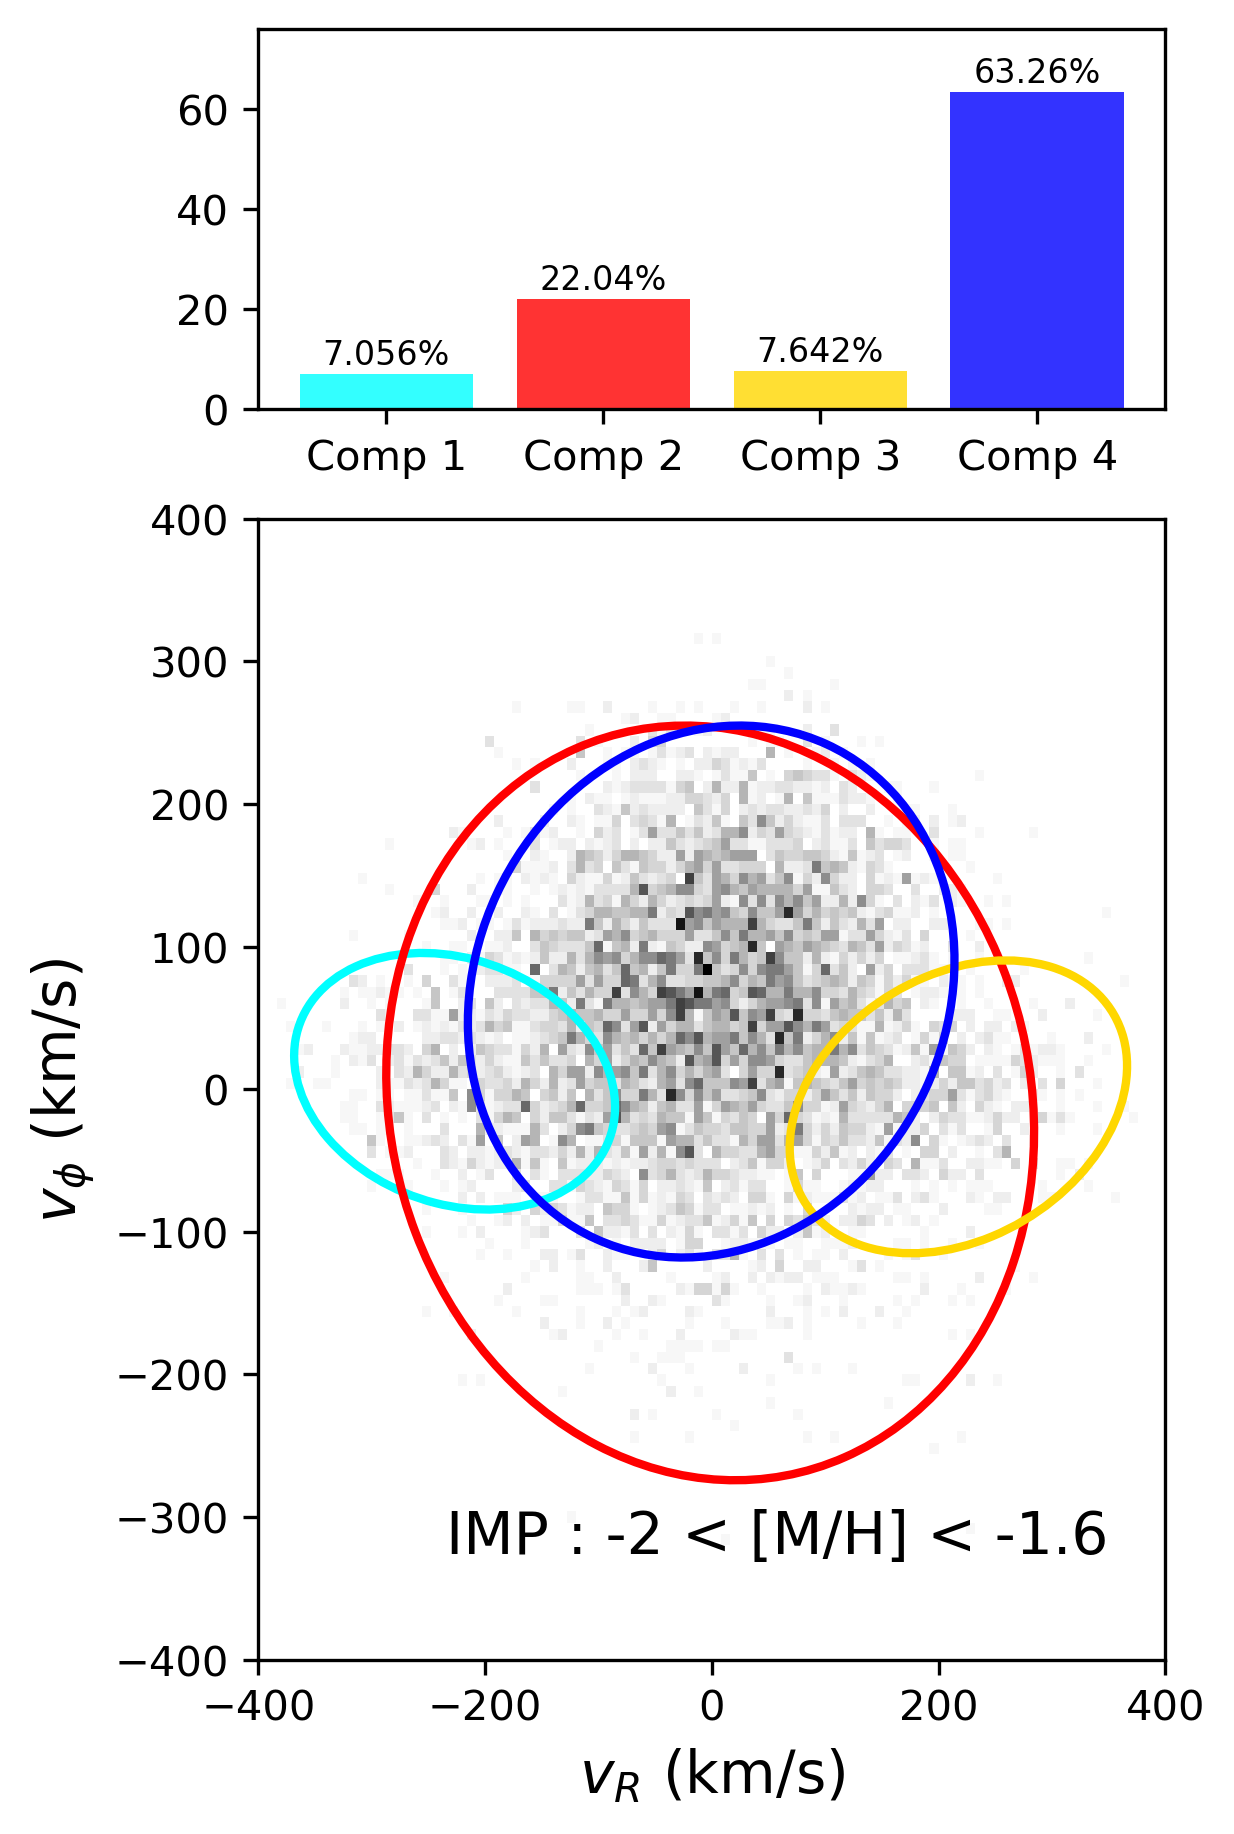
\includegraphics[width=\linewidth]{../figures/gmm_IMP.png}
    \caption{IMP}
    \label{fig:gmm_imp}
  \end{subfigure}
  \hfill
  \begin{subfigure}[t]{0.24\linewidth}
    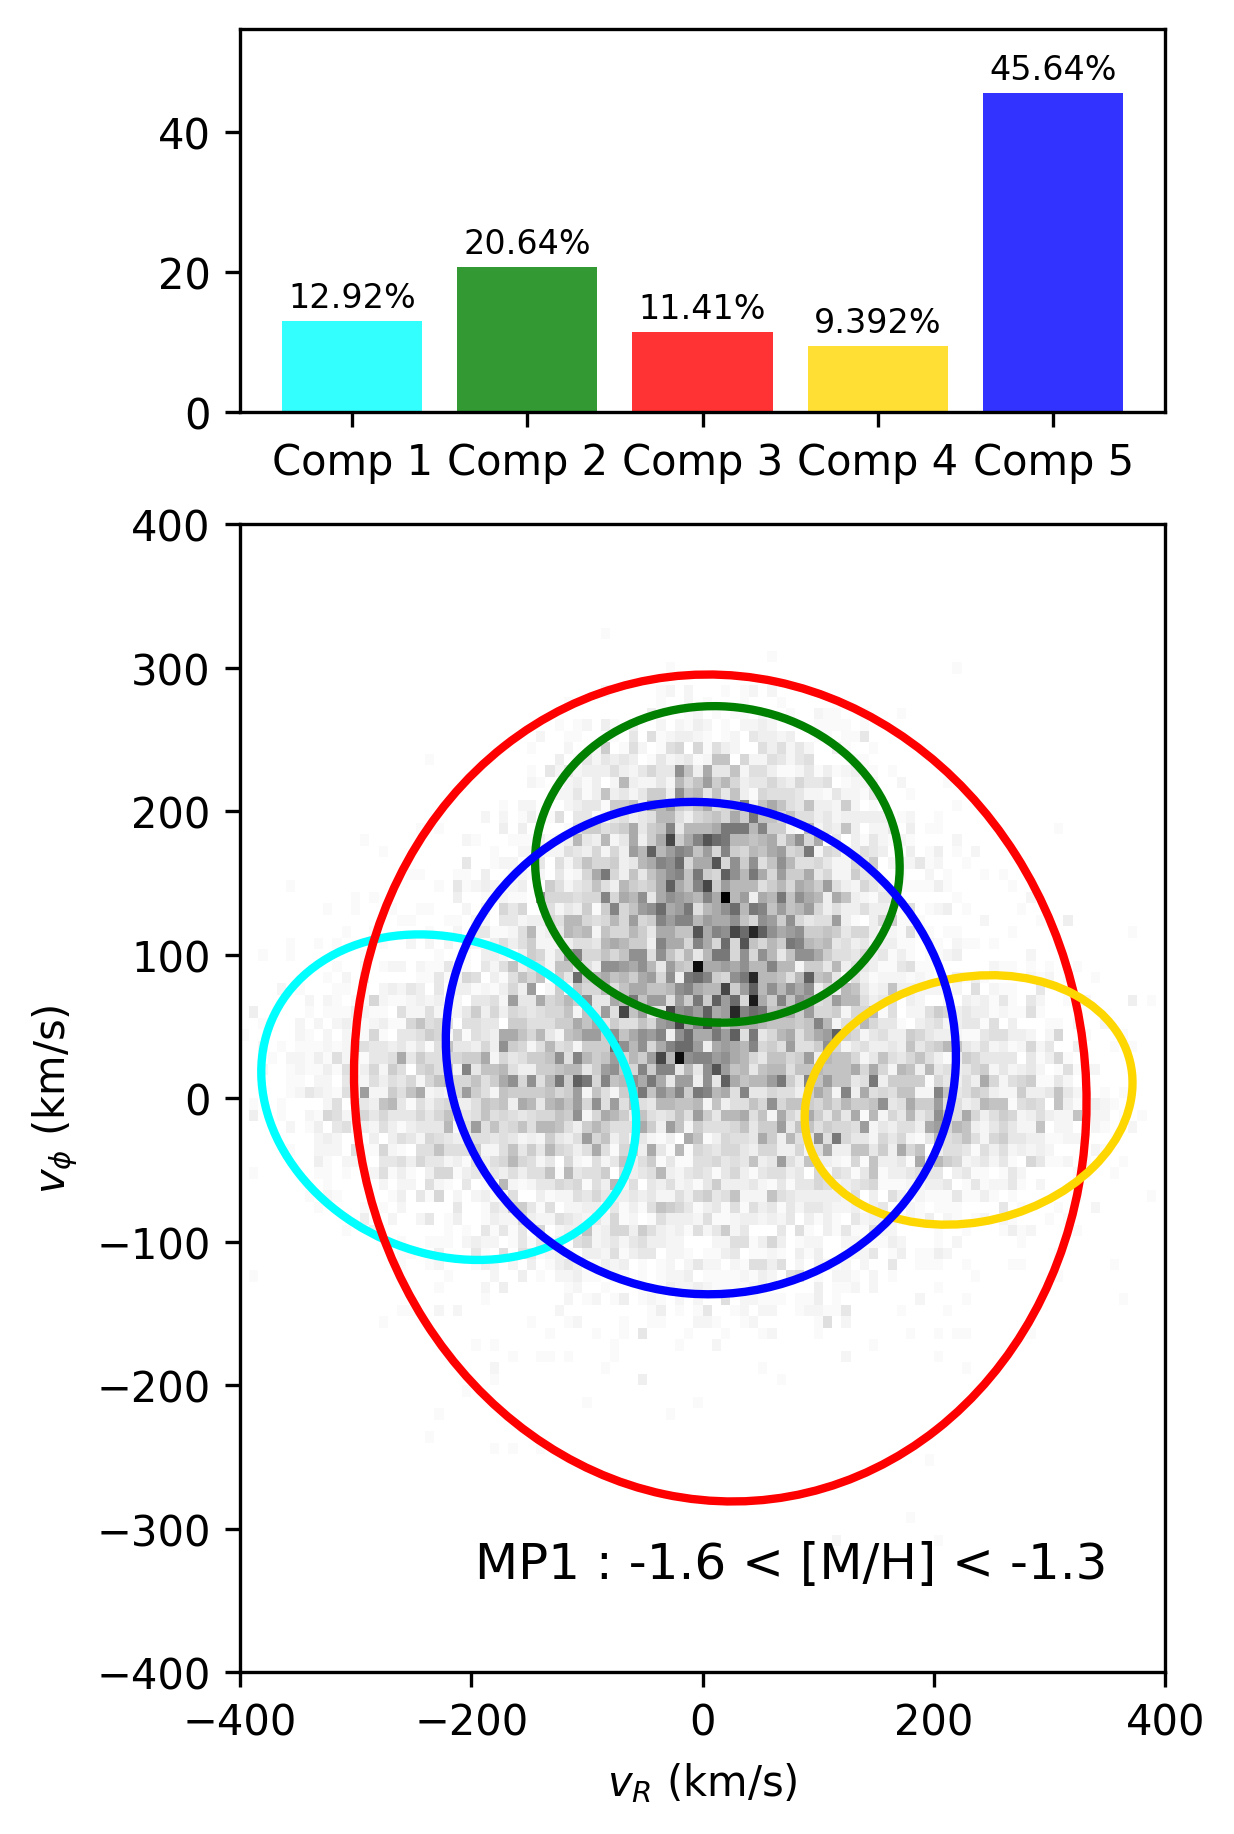
\includegraphics[width=\linewidth]{../figures/gmm_MP1.png}
    \caption{MP1}
    \label{fig:gmm_mp1}
  \end{subfigure}
  \hfill
  \begin{subfigure}[t]{0.24\linewidth}
    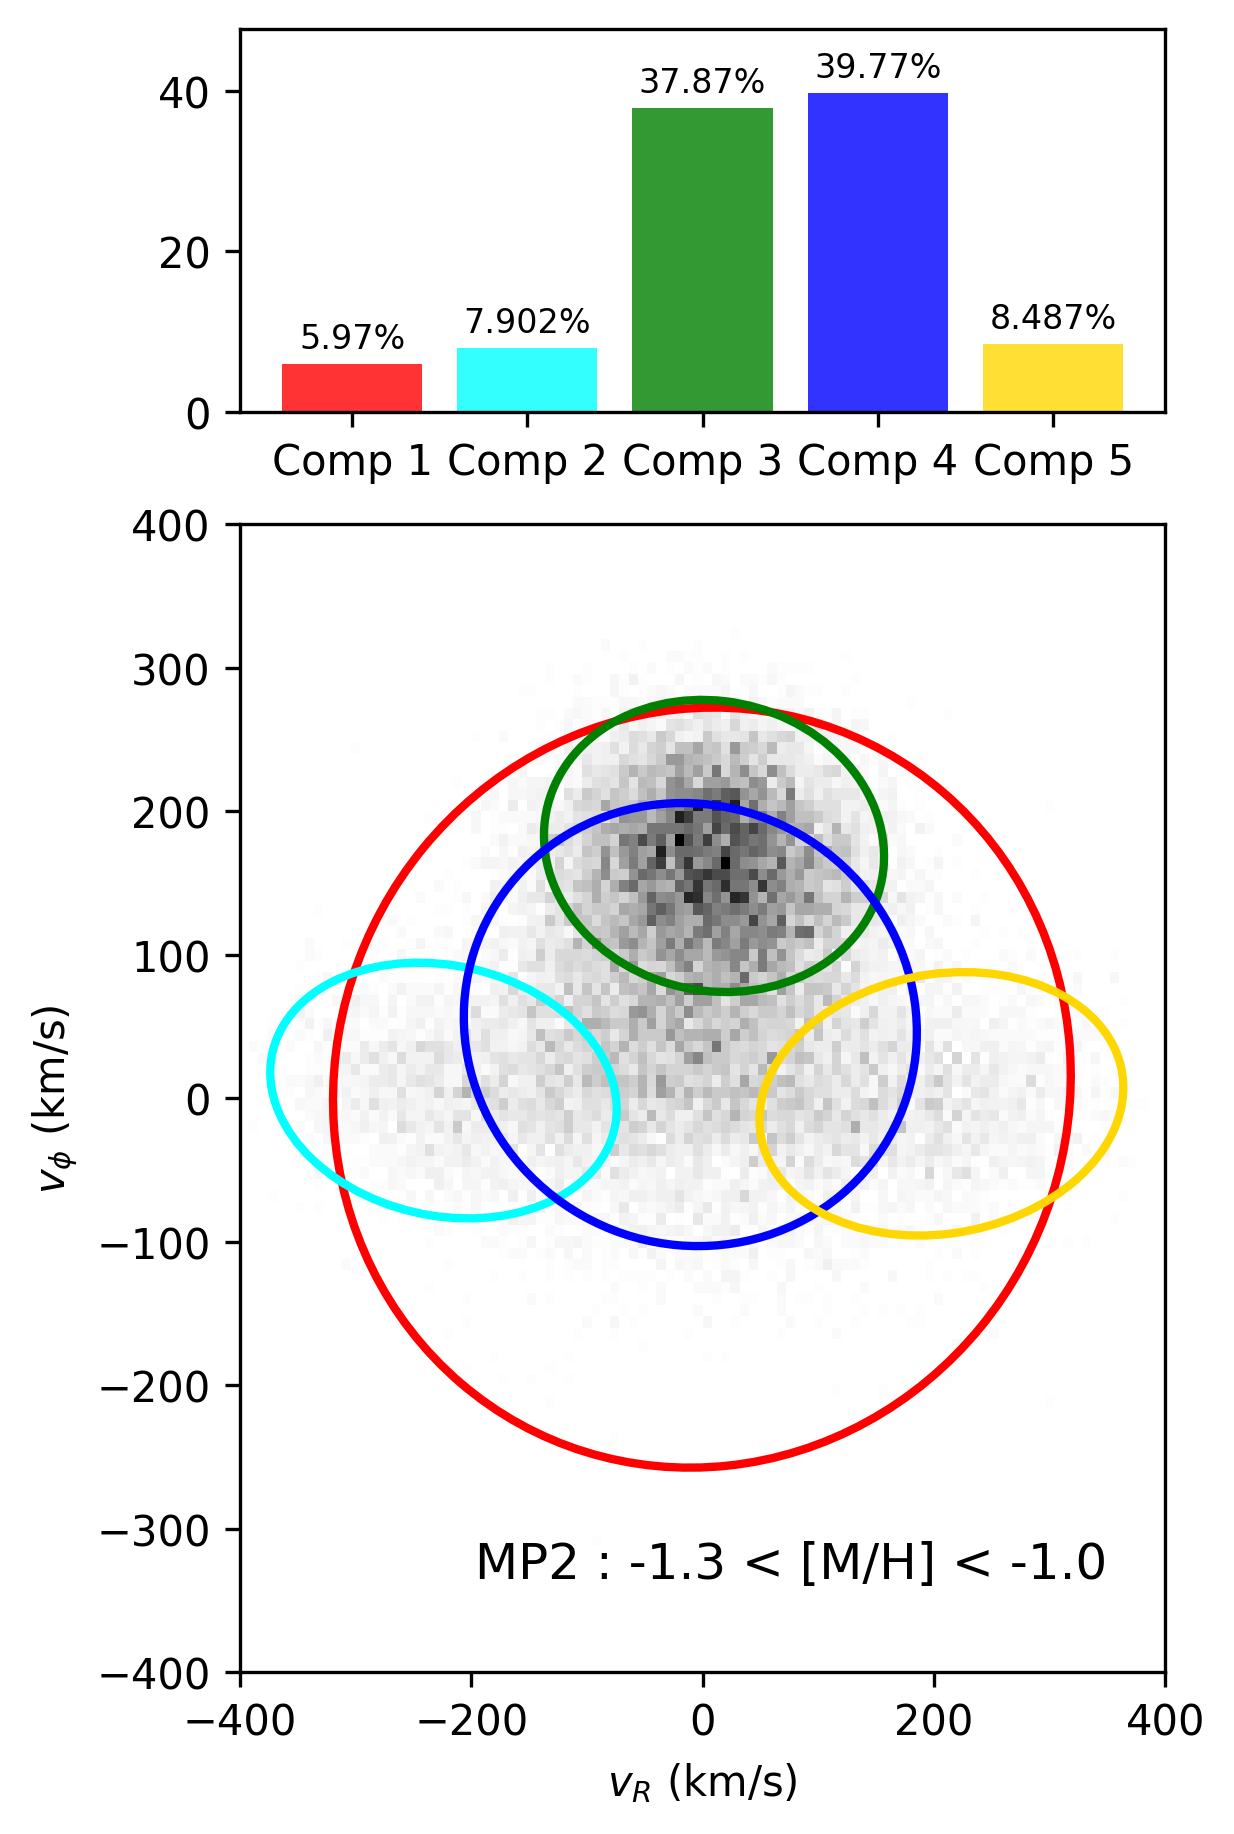
\includegraphics[width=\linewidth]{../figures/gmm_MP2.png}
    \caption{MP2}
    \label{fig:gmm_mp2}
  \end{subfigure}

  \caption{XD–GMM decomposition of red giant kinematics in $v_R$–$v_\phi$ across increasing metallicity bins: very metal-poor (VMP), intermediate (IMP), and two mildly metal-poor bins (MP1, MP2).}
  \label{fig:gmm_zhang}
\end{figure}

\subsection*{Key Findings}

\begin{figure}[H]
  \centering
  \begin{subfigure}[t]{0.24\linewidth}
    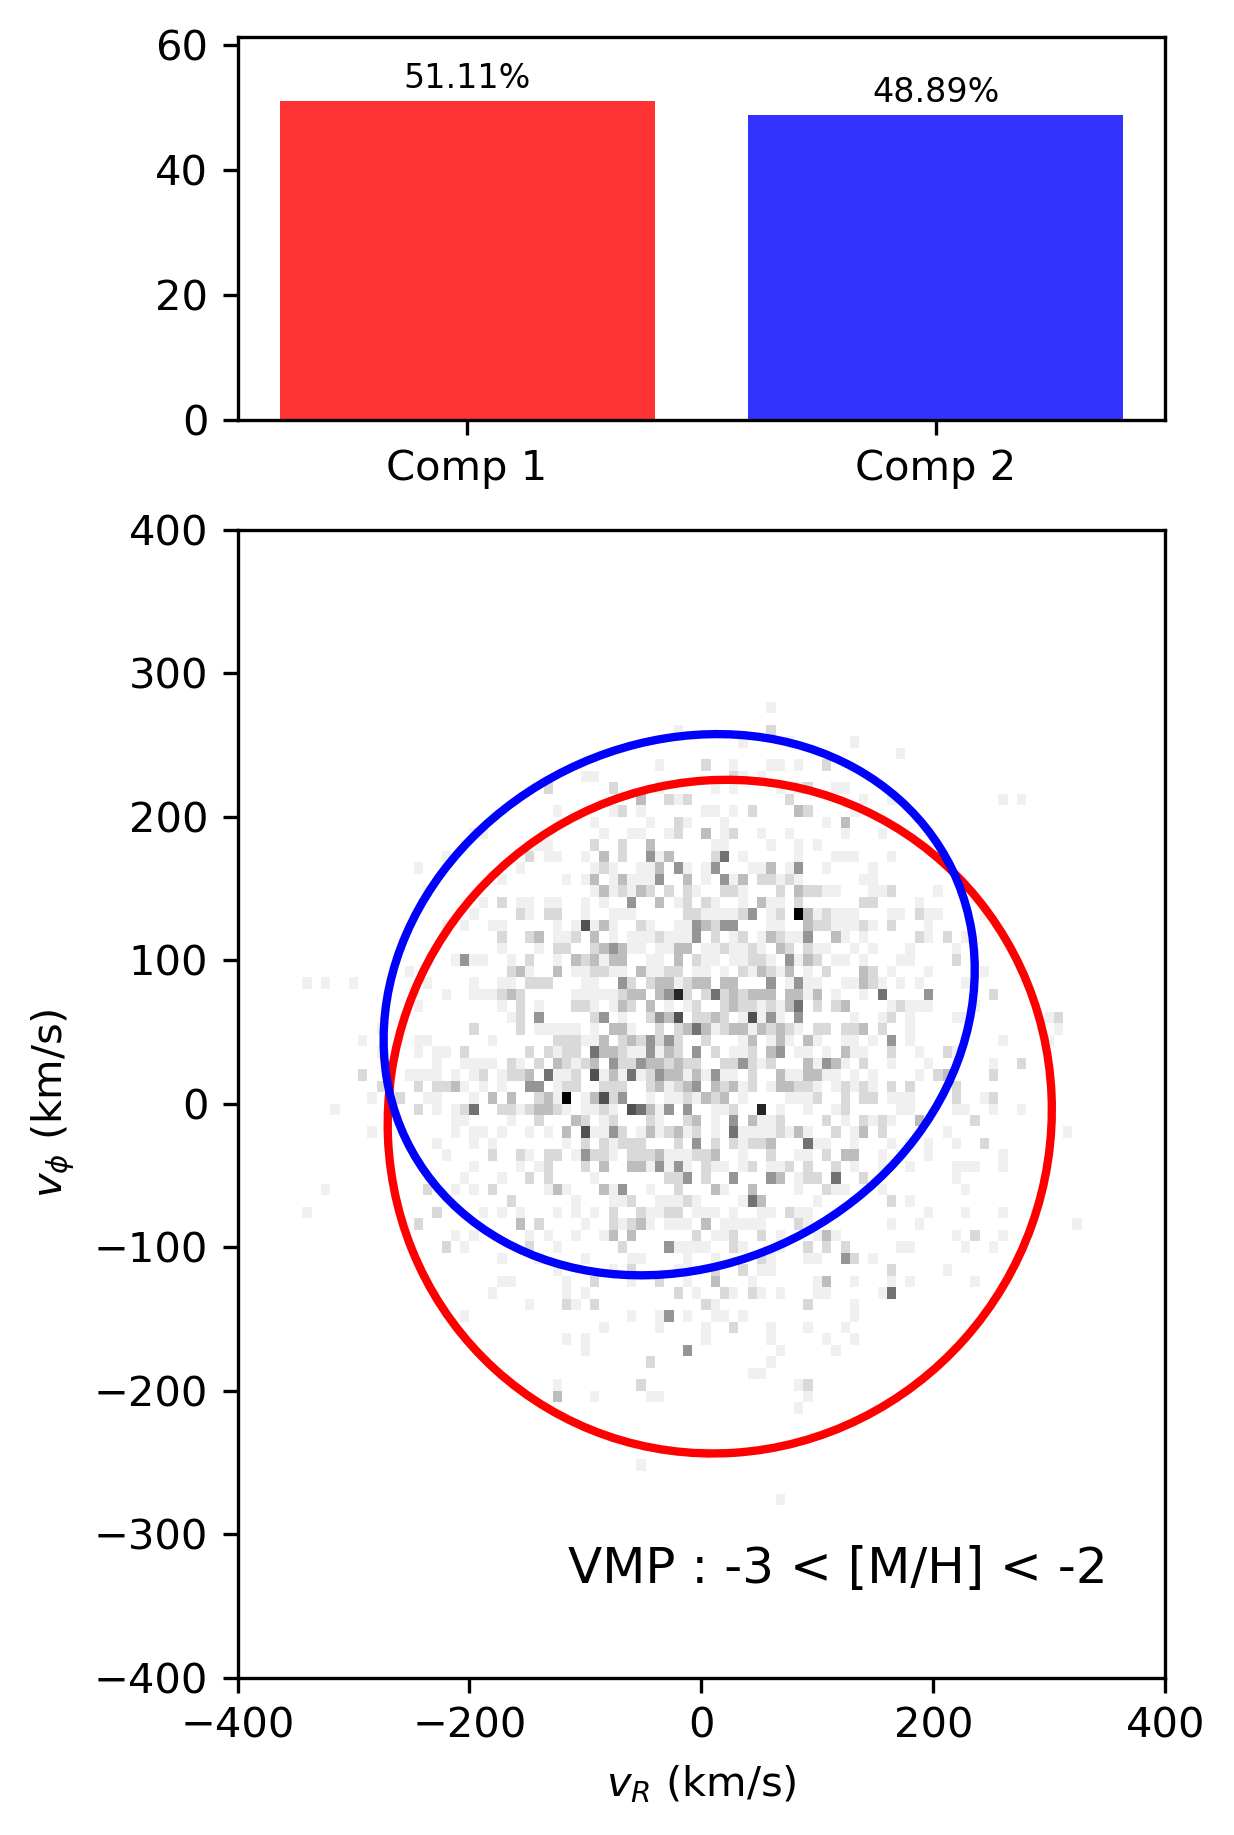
\includegraphics[width=\linewidth]{../figures/gmm_VMP.png}
    \caption{VMP}
    \label{fig:gmm_vmp}
  \end{subfigure}
  \hfill
  \begin{subfigure}[t]{0.24\linewidth}
    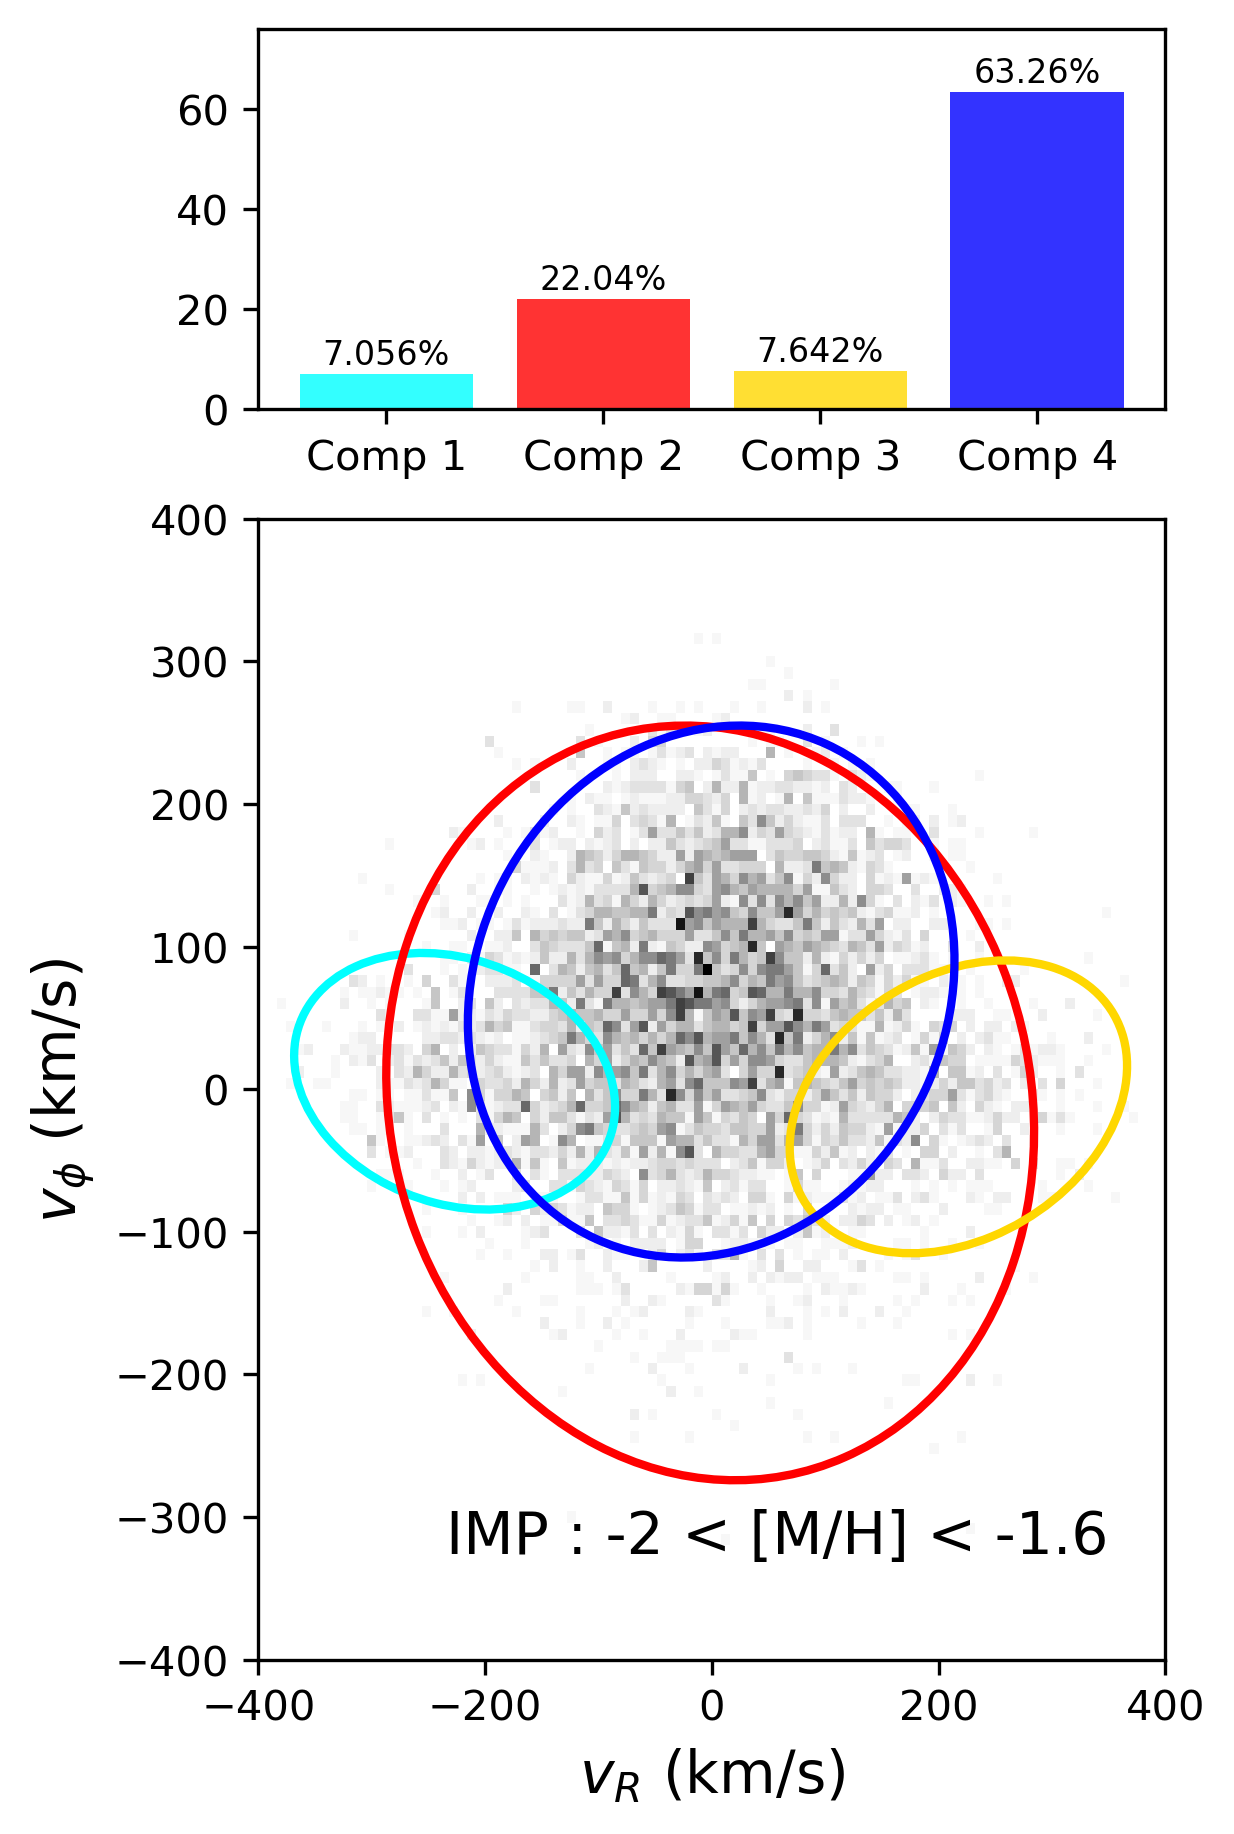
\includegraphics[width=\linewidth]{../figures/gmm_IMP.png}
    \caption{IMP}
    \label{fig:gmm_imp}
  \end{subfigure}
  \hfill
  \begin{subfigure}[t]{0.24\linewidth}
    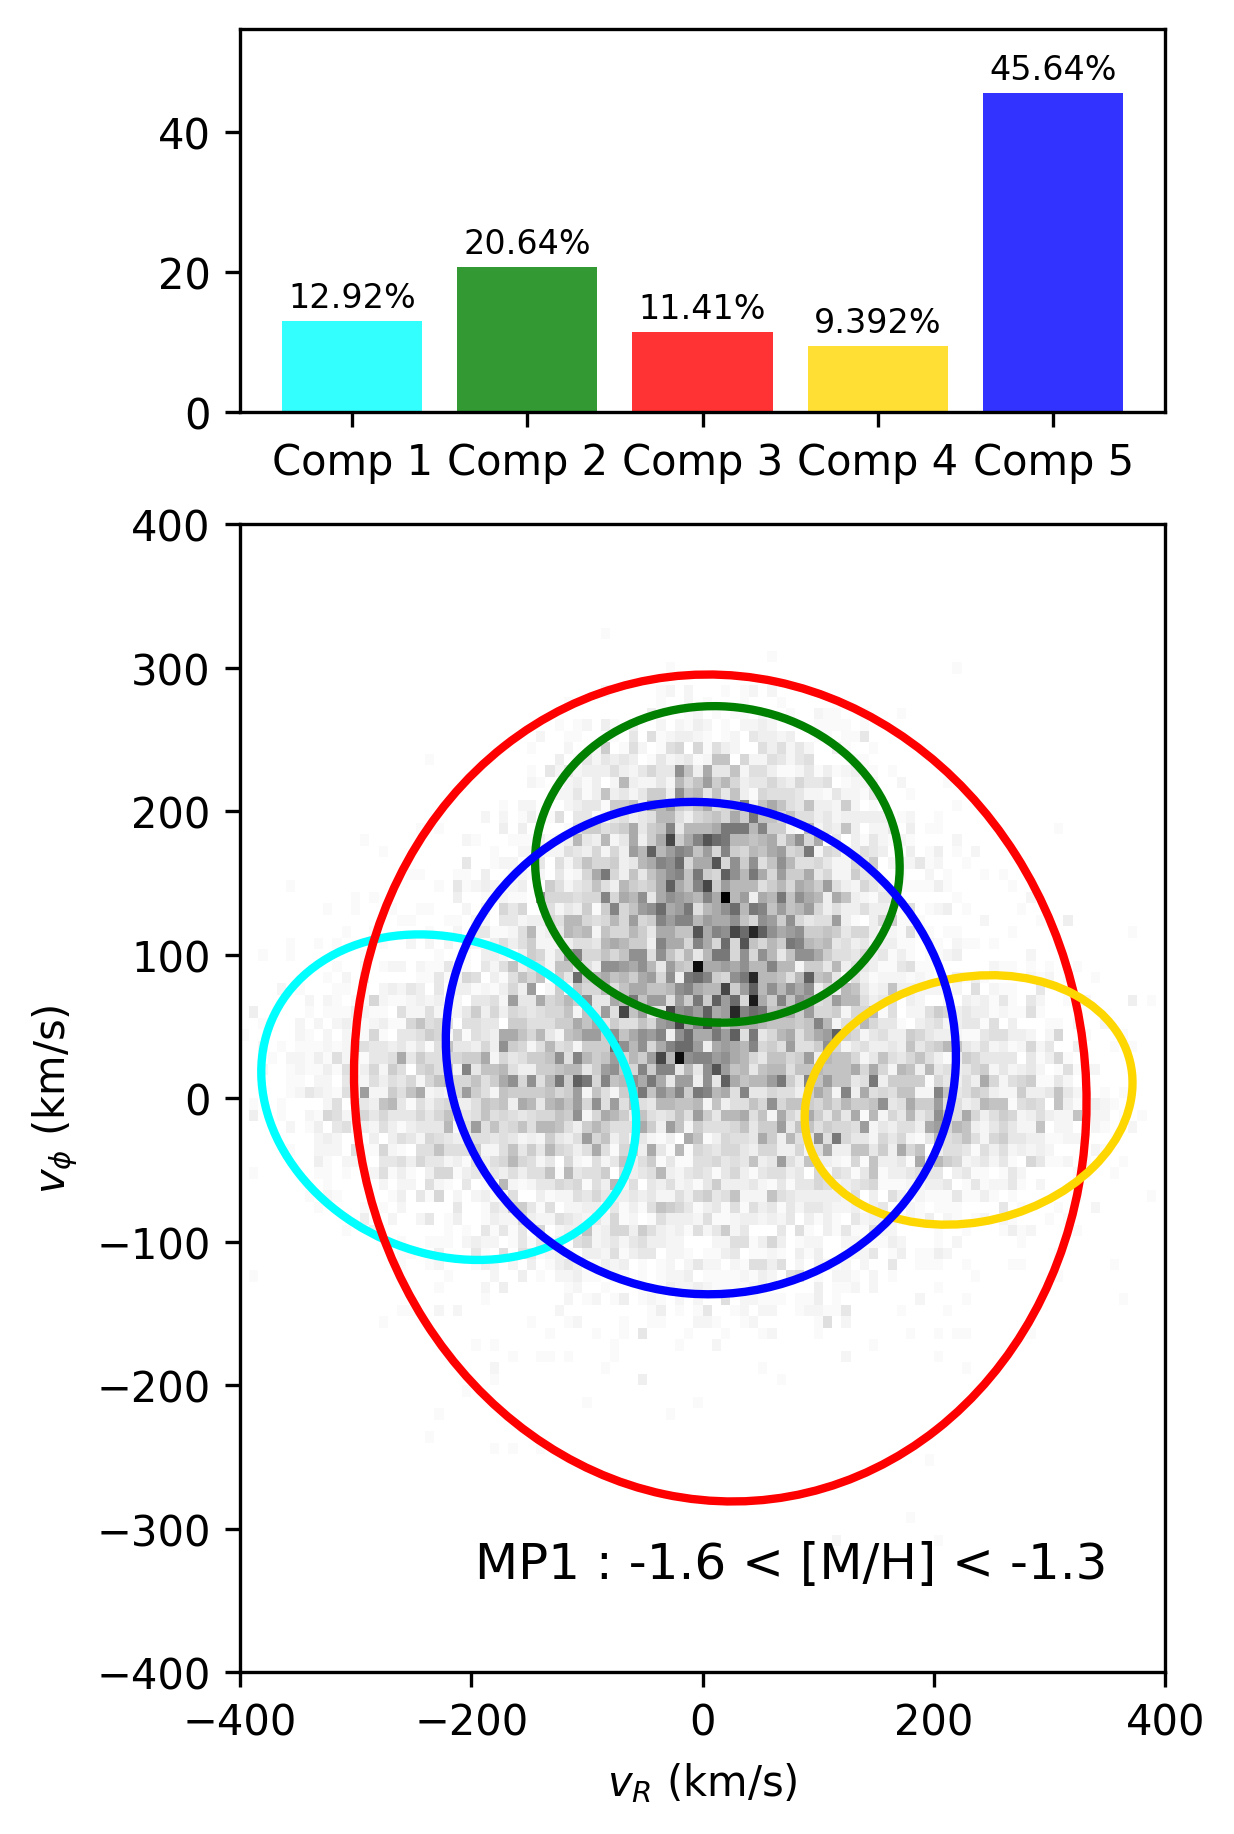
\includegraphics[width=\linewidth]{../figures/gmm_MP1.png}
    \caption{MP1}
    \label{fig:gmm_mp1}
  \end{subfigure}
  \hfill
  \begin{subfigure}[t]{0.24\linewidth}
    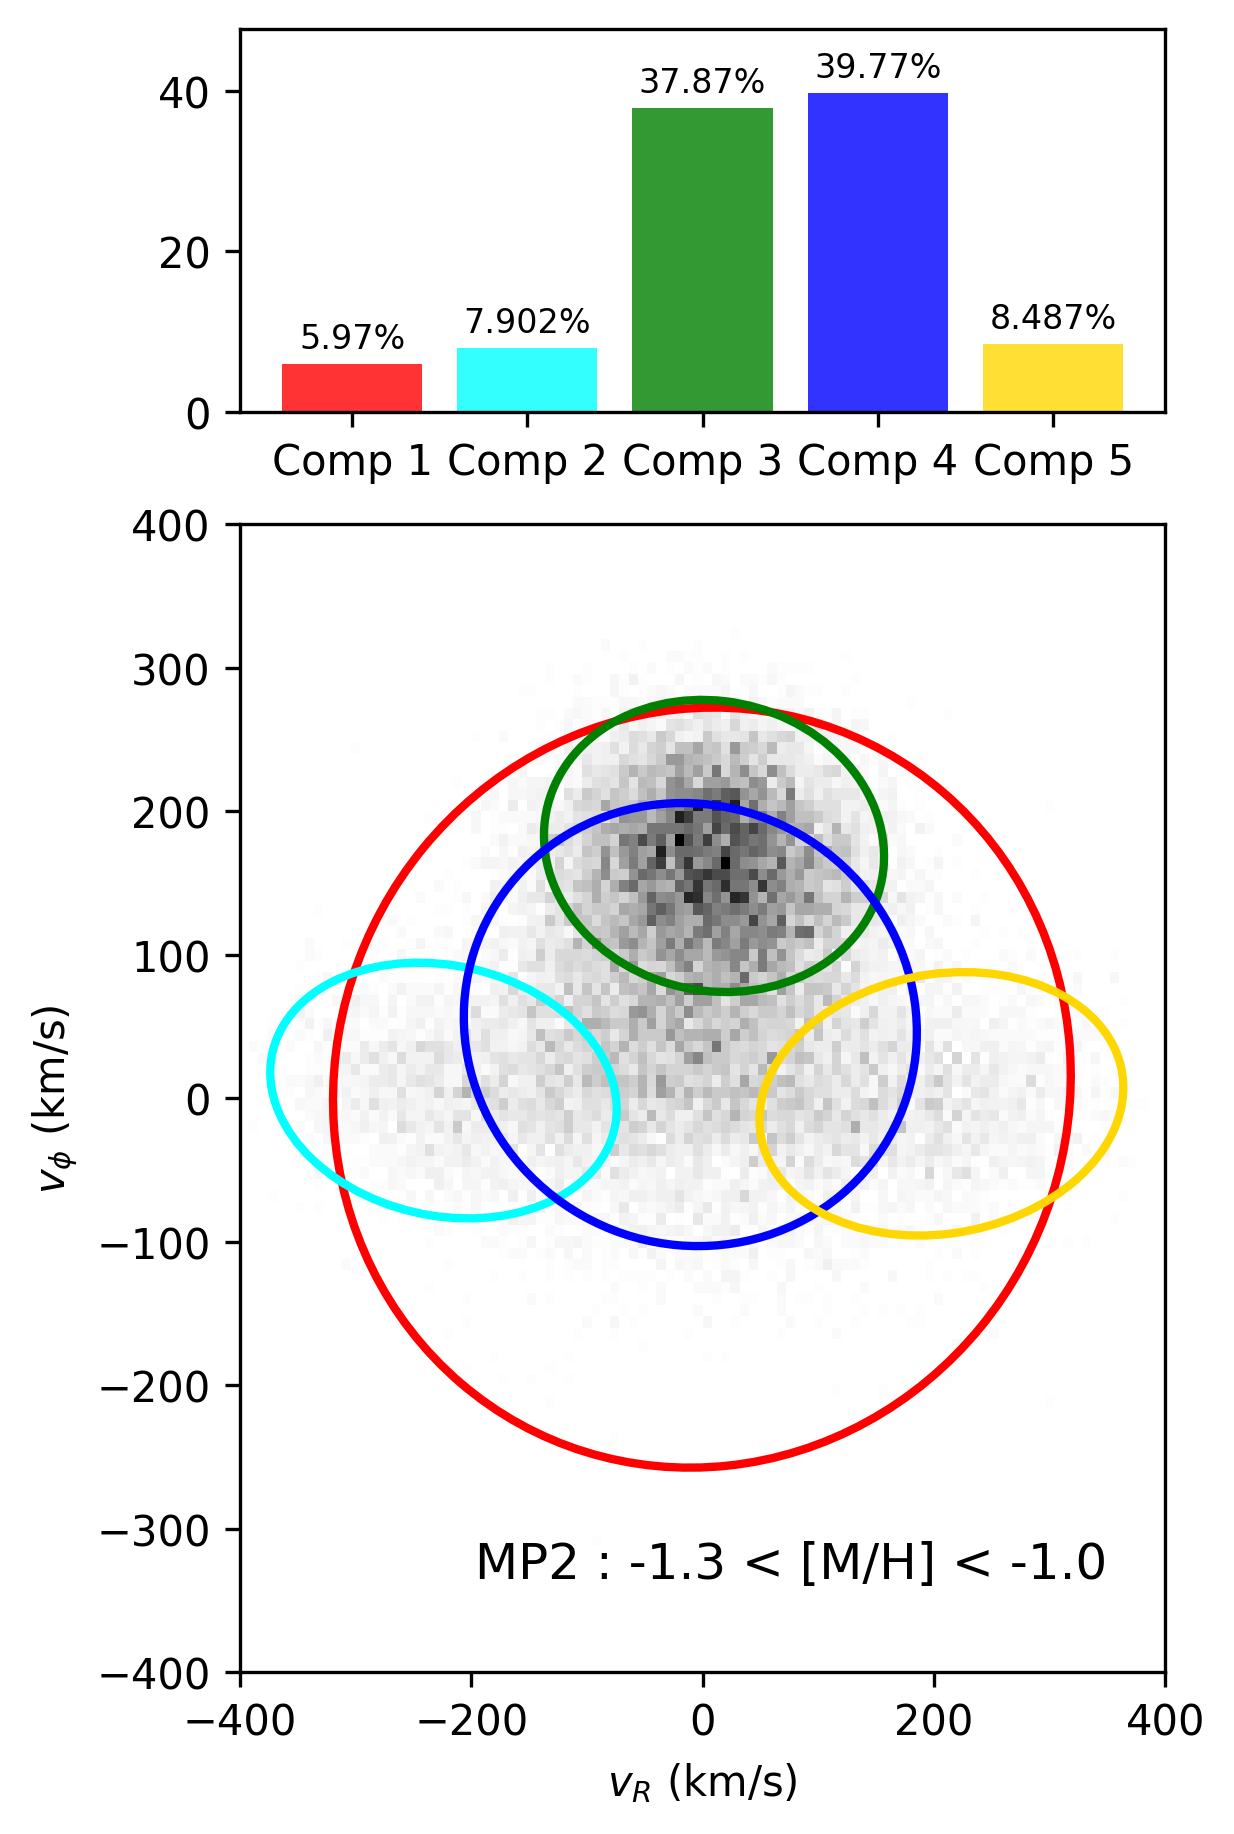
\includegraphics[width=\linewidth]{../figures/gmm_MP2.png}
    \caption{MP2}
    \label{fig:gmm_mp2}
  \end{subfigure}

  \caption{XD–GMM decomposition of red giant kinematics across metallicity bins.}
  \label{fig:gmm_zhang}
\end{figure}

Below $\mathrm{[M/H]} \sim -2$, no disc-like component is detected. The kinematics are fully 
explained by two broad halo Gaussians—one stationary and one mildly prograde whos kinematics 
are likely explained by the Aurora population /cite{Belokurov2022}. In the intermediate 
metallicity bin (IMP), two additional radial components appear, associated with the 
Gaia–Sausage/Enceladus merger /cite{Belokurov2018}. These are highly radial, non-rotating, and contribute 
to halo anisotropy.

Disc-like rotation only emerges above $\mathrm{[M/H]} \sim -1.6$,  
prograde component with relatively low dispersion consistent with an early thick disc. 
This component strengthens with increasing metallicity, supporting a gradual build-up of 
ordered rotation as the Galaxy chemically enriched.

\begin{figure}[H]
  \centering
  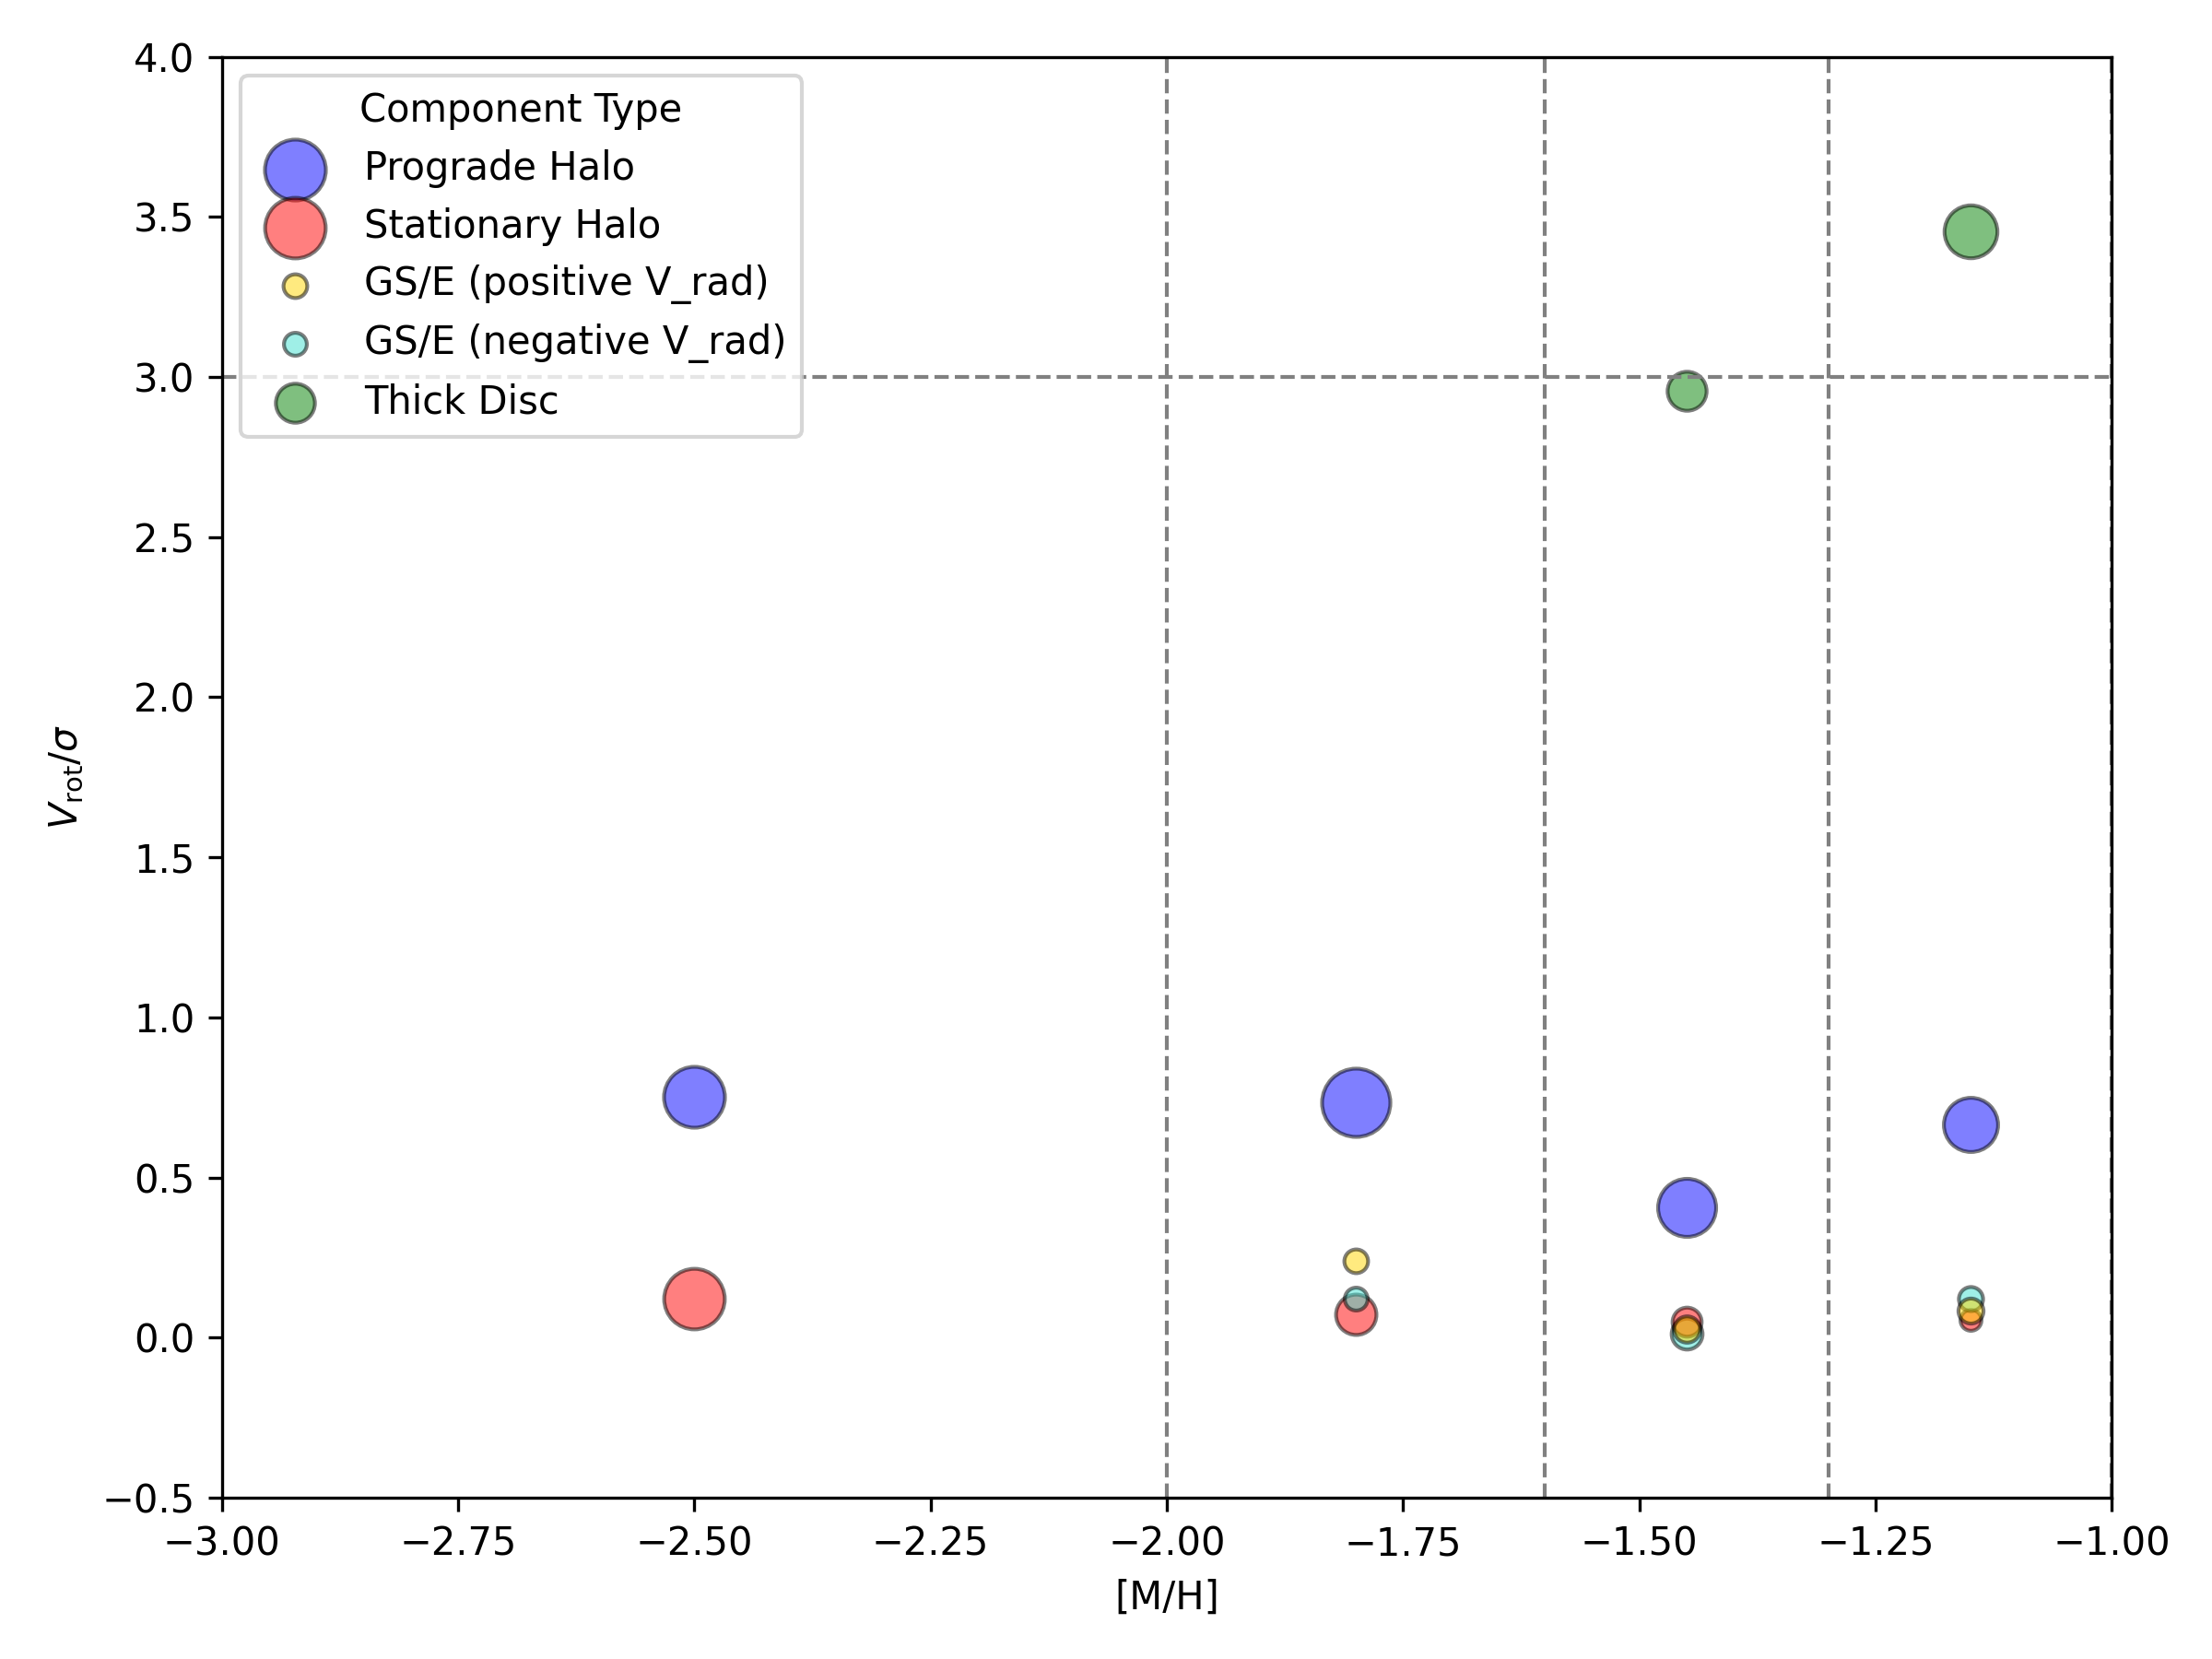
\includegraphics[width=0.6\linewidth]{../figures/v_over_sigma_per_component.png}
  \caption{Rotational support ($v_\phi / \sigma_\phi$) for each Gaussian component across metallicity bins.}
  \label{fig:v_over_sigma}
\end{figure}

As shown in Figure~\ref{fig:v_over_sigma}, stars in the VMP and IMP bins have negligible rotational support, 
with $v_\phi / \sigma_\phi < 1$. It is generally accepted that a disc-like population should have 
$v_\phi / \sigma_\phi \gg 1$, confirming the absence of a cold disc for $\mathrm{[M/H]} < -1.6$.











\bibliographystyle{unsrt}  % Or use apalike, mnras, etc., depending on your needs
\bibliography{references}

% End of two-column content
\end{multicols}



\end{document}
